\documentclass{article}
\usepackage{indentfirst}
\usepackage{framed}
\usepackage{amsmath}
\usepackage{tikz}
\usepackage{tikz-3dplot}
% \usepackage{esvect}
\usepackage{cancel}
\usepackage{float}
\usepackage{comment}
\usepackage{graphicx}
\graphicspath{ {./Figures/} }

\usepackage[pdfencoding=auto, psdextra]{hyperref}
\hypersetup{
    colorlinks = true, %Colours links instead of ugly boxes
    urlcolor = blue, %Colour for external hyperlinks
    linkcolor = blue, %Colour of internal links
}

\usepackage[a4paper, left=3.5cm,right=3.5cm, top=3cm, bottom=3cm]{geometry}

\newcommand{\dd}[2]{\frac{\mathrm{d}#1}{\mathrm{d}#2}}
\newcommand{\vv}[1]{\boldsymbol{#1}}
\newcommand{\vh}[1]{\boldsymbol{\hat{#1}}}


\title{Multibody Dynamics Primer}
\author{Polaris}
\date{}

\begin{document}
\maketitle

\pagebreak

% \section*{Diagrams}
The circular restricted three body problem (CR3BP) is a special case of the three body problem. In the CR3BP (much like in Keplerian 2-body dynamics), we neglect the mass of satellite $S$, while treating the larger celestial body $m_1$ and smaller celestial body $m_2$ as point masses. Crucially, these bodies must orbit one another in circular orbits. In other words, they both orbit about their inertially fixed barycenter $c$ \textit{at constant velocity and distance}.

\begin{figure}[H]
    \centering
    \tdplotsetmaincoords{70}{30}
    \begin{tikzpicture}[
        planet/.style = {circle, draw=black, ball color=#1, node contents={}, inner sep = 0.1cm}, 
        point/.style = {circle, draw=#1, fill=#1, node contents={}, inner sep=0.05cm},
        >=latex,
        tdplot_main_coords
        ]

        \node (B1) at (-1,0,0)     [planet=red, label=left:$m_1$];
        \node (B2) at (3,0,0)      [planet=blue, label=right:$m_2$];
        \draw[dashed, <->, lightgray] (-1,0,-1) -- (3,0,-1) node[midway, below] {$d$};
        \draw[dotted, thin, lightgray] (B1) -- ++(0,0,-1);
        \draw[dotted, thin, lightgray] (B2) -- ++(0,0,-1);
        
        \draw[dash dot, fill=none, red](0,0,0) circle (1);
        \draw[dash dot, fill=none, blue](0,0,0) circle (3);

        \draw[dashed, red] (B1) -- (0,0,0) node[midway] {$x_1$};
        \draw[dashed, blue] (0,0,0) -- (B2) node[midway] {$x_2$};
        
        \node (o) at (0,0,0)      [point=black, label=below:$c$];
        \node (r) at (1.25,2,1.25)    [point=purple, label=left:$S$];
        \draw[dashed, purple] (0,0,0) -- (0, 2, 0) node[midway, right]  {$y$} -- (1.25, 2, 0) node[midway, above]  {$x$} -- (r) node[midway, right] {$z$};

        \draw[->, gray] (0,0,0) -- (0.75,0,0) node[near end, below right] {$\vh{x}$};
        \draw[->, gray] (0,0,0) -- (0,0.75,0) node[near end, above] {$\vh{y}$};
        \draw[->, gray] (0,0,0) -- (0,0,0.75) node[near end, above left] {$\vh{z}$};

        \draw[dashed, gray] (0,0,0) -- (0,0,2);
        \draw[->, gray] (0.5,0,2) arc (0:270:0.5) node [midway, above] {$\Omega$};
    \end{tikzpicture}

    \caption{Geometry}
\end{figure}

The purple satellite is located by $\vv{r}=x\vh{x}+y\vh{y}+z\vh{z}$, and the spheres are the celestial bodies. The $xyz$ frame is not inertially stationary. Instead, they rotate with the larger bodies at a rate $\Omega$. The origin $c$ is the center of mass of $m_1$ and $m_2$ (and therefore inertially fixed). The $xy$ plane defines the plane in which $m_1$ and $m_2$ orbit, so $\vh{z}$ is defined by the direction of their angular momenta- the constant rotation at a rate $\Omega$ is a consequence of this. Note that $\vv{r}$ is not constrained to the $xy$ plane, but $m_1$ and $m_2$ definitionally are. 

\section*{Useful Relations}

We can also find a relationship between $x_1$, $x_2$, $d$, $m_1$, and $m_2$. Because $c$ is the barycenter,
\[x_1m_1=x_2m_2\]
or
\[\frac{x_1}{m_2}=\frac{x_2}{m_1}\]
We can use this to find that
\[\begin{aligned}
\frac{x_1}{x_1+x_2}&=\frac{x_1/m_2}{x_1/m_2+x_2/m_2}\\
&=\frac{x_2/m_1}{x_2/m_1+x_2/m_2}\\
&=\frac{1/m_1}{1/m_1+1/m_2}\\
&=\frac{m_2}{m_2+m_1}\\
\end{aligned}\]

Defining $d=x_1+x_2$ as the distance between the two celestial bodies, and $m=m_1+m_2$ as their total mass, we get that
\[\boxed{\frac{x_1}{d}=\frac{m_2}{m}}\]
and similarly
\[\boxed{\frac{x_2}{d}=\frac{m_1}{m}}\]


Which can be rewritten as
\[\boxed{\frac{x_1}{m_2}=\frac{x_2}{m_1}=\frac{d}{m}}\]

Lastly, we will define two additional vectors $\vv{r_1}$ and $\vv{r_2}$ which point from the first and second body respectively to the satellite.
\[\vv{r_1}=\left(x+x_1\right)\vh{x}+y\vh{y}+z\vh{z}\]
and
\[\vv{r_2}=\left(x-x_2\right)\vh{x}+y\vh{y}+z\vh{z}\]

Now we will solve for $\Omega$.
\[\begin{aligned}
    \vv{F_{\text{on2}}}&=-\frac{Gm_1m_2}{d^2}\vh{x}\\
    \cancel{m_2}\vv{a}_2^f&=-\frac{Gm_1\cancel{m_2}}{d^2}\vh{x}\\
    \dd{^f}{t}\left(\dd{^f}{t}x_2\vh{x}\right)&=-\frac{Gm_1}{d^2}\vh{x}\\
    \dd{^f}{t}\left(\cancelto{0}{\dd{^c x_2\vh{x}}{t}}+\Omega\vh{z}\times x_2\vh{x}\right)&=-\frac{Gm_1}{d^2}\vh{x}\\
    \dd{^f}{t}\Omega x_2\vh{y}&=-\frac{Gm_1}{d^2}\vh{x}\\
    \cancelto{0}{\dd{^c}{t}\Omega x_2 \vh{y}}+\Omega\vh{z}\times\Omega x_2\vh{y}&=-\frac{Gm_1}{d^2}\vh{x}\\
    -\Omega^2 x_2\vh{x}&=-\frac{Gm_1}{d^2}\vh{x}\\
    \Omega^2x_2&=\frac{Gm_1}{d^2}\\
    \Omega&=\sqrt{\frac{G}{d^2}\frac{m_1}{x_2}}\\
    \Omega&=\sqrt{\frac{Gm}{d^3}}\\
\end{aligned}\]

\[\boxed{\Omega=\sqrt{\frac{Gm}{d^3}}}\]

\section*{Kinematics}
The transport theorem states that the inertial (fixed $f$ frame) derivative of a vector $u$ (expressed in the rotating $c$ frame) is

\[\dd{^f \vv{u}}{t}=\dd{^c\vv{u}}{t}+\vv{\omega}^{cf}\times\vv{u}\]

Where $\dd{^f}{t}$ denotes the derivative in the coordinates of the fixed frame $f$, and $\dd{^c}{t}$ denotes derivative in the coordinates of the rotating frame $c$, and $\vv{\omega}^{cf}$ denotes the angular velocity of $c$ in $f$. For this case, $\vv{\omega}^{cf}=\Omega\vh{z}$. We can find $\Omega$

For the satellite's position in the CR3BP frame $\vv{r}=x\vh{x}+y\vh{y}+z\vh{z}$, we will find the inertial acceleration to generate equations of motion.

\[
\begin{aligned}
    \vv{\dot{r}}&=\dd{^c\vv{r}}{t}+\vv{\omega}^{cf}\times\vv{r}\\
    &=\dd{^c}{t}\left(x\vh{x}+y\vh{y}+z\vh{z}\right)+\left(\Omega\vh{z}\times\left(x\vh{x}+y\vh{y}+z\vh{z}\right)\right)\\
    &=\left(\dot{x}\vh{x}+\dot{y}\vh{y}+\dot{z}\vh{z}\right)+\left(\Omega x\vh{y}-\Omega y\vh{x}\right)\\
    &=\left(\dot{x}-\Omega y\right)\vh{x}+\left(\dot{y}+\Omega x\right)\vh{y}+\dot{z}\vh{z}
\end{aligned}
\]

\[
\begin{aligned}
    \vv{\ddot{r}}&=\dot{\vv{r}}\\
    &=\dd{^c}{t}\left(\left(\dot{x}-\Omega y\right)\vh{x}+\left(\dot{y}+\Omega x\right)\vh{y}+\dot{z}\vh{z}\right)\\
        &\phantom{=}\quad+\Omega \vh{z}\times\left(\left(\dot{x}-\Omega y\right)\vh{x}+\left(\dot{y}+\Omega x\right)\vh{y}+\dot{z}\vh{z}\right)\\
    &=\left(\ddot{x}-\Omega \dot{y}\right)\vh{x}+\left(\ddot{y}+\Omega \dot{x}\right)\vh{y}+\ddot{z}\vh{z}\\
        &\phantom{=}\quad+\left(\left(\Omega\dot{x}-\Omega^2 y\right)\vh{y}-\left(\Omega\dot{y}+\Omega^2 x\right)\vh{x}\right)\\
    &=\left(\ddot{x}-2\Omega\dot{y}-\Omega^2 x\right)\vh{x} + \left(\ddot{y}+2\Omega\dot{x}-\Omega^2 y\right)\vh{y}+\ddot{z}\vh{z}\\
\end{aligned}
\]

\[\boxed{\vv{\ddot{r}}=\left(\ddot{x}-2\Omega\dot{y}-\Omega^2 x\right)\vh{x} + \left(\ddot{y}+2\Omega\dot{x}-\Omega^2 y\right)\vh{y}+\ddot{z}\vh{z}}\]

Or, rewritten,
\[\begin{aligned}
    \vv{\ddot{r}} & = \left(\ddot{x}-2\Omega\dot{y}-\Omega^2 x\right)\vh{x} + \left(\ddot{y}+2\Omega\dot{x}-\Omega^2 y\right)\vh{y}+\ddot{z}\vh{z}\\
    \vv{\ddot{r}} & = \left(\ddot{x}\vh{x}+\ddot{y}\vh{y}+\ddot{z}\vh{z}\right) - \Omega^2\left(x\vh{x}+y\vh{y}\right)-2\Omega\dot{y}\vh{x} + 2\Omega\dot{x}\vh{y}\\
    \vv{\ddot{r}} & = \vv{a^c} - \Omega^2\vv{r_{xy}} + 2\vv{\Omega}\times\vv{v^c}\\
\end{aligned}\]

\[\boxed{\vv{\ddot{r}} = \underbrace{\vv{a^c}}_\text{Relative Acceleration} + \overbrace{- \Omega^2\vv{r_{xy}}}^\text{Centripedal Acceleration} + \underbrace{2\vv{\Omega}\times\vv{v^c}}_\text{Coriolis Acceleration}}\]
\section*{Equations of Motion}
We can now generate the equations of motion

\[\begin{aligned}
\sum_i \vv{F_i}&=m\vv{\ddot{r}}\\
\vv{F_1}+\vv{F_1}&=m\vv{\ddot{r}}\\
-\frac{Gm_1m}{r_1^3}\vv{r_1}-\frac{Gm_2m}{r_2^3}\vv{r_2}&=m\vv{\ddot{r}}\\
-\frac{Gm_1}{r_1^3}\vv{r_1}-\frac{Gm_2}{r_2^3}\vv{r_2}&=\left(\ddot{x}-2\Omega\dot{y}-\Omega^2 x\right)\vh{x} + \left(\ddot{y}+2\Omega\dot{x}-\Omega^2 y\right)\vh{y}+\ddot{z}\vh{z}
\end{aligned}\]

We now write this as three equations, one each in $x$, $y$, and $z$
\[\begin{aligned}
    -\frac{Gm_1}{r_1^3}(x+x_1)-\frac{Gm_2}{r_2^3}(x-x_2)&=\ddot{x}-2\Omega\dot{y}-\Omega^2 x\\
    -\frac{Gm_1}{r_1^3}y-\frac{Gm_2}{r_2^3}y&=\ddot{y}+2\Omega\dot{x}-\Omega^2 y\\
    -\frac{Gm_1}{r_1^3}z-\frac{Gm_2}{r_2^3}z&=\ddot{z}
\end{aligned}\]

Isolating the second derivatives,

\[\begin{aligned}
    \ddot{x}&=-\frac{Gm_1}{r_1^3}(x+x_1)-\frac{Gm_2}{r_2^3}(x-x_2)+2\Omega\dot{y}+\Omega^2 x\\
    \ddot{y}&=-\frac{Gm_1}{r_1^3}y-\frac{Gm_2}{r_2^3}y-2\Omega\dot{x}+\Omega^2 y\\
    \ddot{z}&=-\frac{Gm_1}{r_1^3}z-\frac{Gm_2}{r_2^3}z
\end{aligned}\]
    
We can now substitute $\Omega=\sqrt{\frac{Gm}{d^3}}=\sqrt{\frac{Gm_1+Gm_2}{d^3}}$

\[\boxed{\begin{aligned}
    \ddot{x}&=-\frac{Gm_1}{r_1^3}(x+x_1)-\frac{Gm_2}{r_2^3}(x-x_2)+2\sqrt{\frac{Gm}{d^3}}\dot{y}+\frac{Gm}{d^3}x\\
    \ddot{y}&=-\frac{Gm_1}{r_1^3}y-\frac{Gm_2}{r_2^3}y-2\sqrt{\frac{Gm}{d^3}}\dot{x}+\frac{Gm}{d^3}y\\
    \ddot{z}&=-\frac{Gm_1}{r_1^3}z-\frac{Gm_2}{r_2^3}z
\end{aligned}}\]

\section*{Nondimensional Equations of Motion}
We will now begin to non-dimensionalize the EOMs.

First, we will change the time unit. We will pick $t^\star=t\sqrt{Gm/d^3}$ (recall that $\sqrt{Gm/d^3}=\Omega$, which has dimensions of $\text{time}^{-1}$). Everywhere that a derivative is present, it is implied to be with respect to the time unit of 1 second. We must therefore switch from implied $\dd{}{t}$ to implied $\dd{}{t^\star}$.

\[\begin{aligned}
    \dd{(\phantom{x})}{t}&=\dd{(\phantom{x})}{t^\star}\dd{t^\star}{t}\\
    &=\dd{(\phantom{x})}{t^\star}\sqrt{\frac{Gm}{d^3}}
\end{aligned}\]

From this, it can be seen that to make a derivative with time implied to be with the nondimensional time, $\sqrt{d^3/Gm}$ must be multiplied for each derivative taken. The EOMs can now be rewritten this way, with dots implied to be relative to the nondimensional time unit

\[\begin{aligned}
    \left(\dd{^2x}{t^{\star2}}\frac{Gm}{d^3}\right)&=-\frac{Gm_1}{r_1^3}(x+x_1)-\frac{Gm_2}{r_2^3}(x-x_2)+2\sqrt{\frac{Gm}{d^3}}\left(\dd{y}{t^\star}\sqrt{\frac{Gm}{d^3}}\right)+\frac{Gm}{d^3}x\\
    \left(\dd{^2y}{t^{\star2}}\frac{Gm}{d^3}\right)&=-\frac{Gm_1}{r_1^3}y-\frac{Gm_2}{r_2^3}y-2\sqrt{\frac{Gm}{d^3}}\left(\dd{x}{t^\star}\sqrt{\frac{Gm}{d^3}}\right)+\frac{Gm}{d^3}y\\
    \left(\ddot{z}\frac{Gm}{d^3}\right)&=-\frac{Gm_1}{r_1^3}z-\frac{Gm_2}{r_2^3}z
\end{aligned}\]

Some algebraic simplifications can now be made

\[\begin{aligned}
    \dd{^2x}{t^{\star2}}&=-\frac{m_1 d^3}{m r_1^3}(x+x_1)-\frac{m_2 d^3}{m r_2^3}(x-x_2)+2\dd{y}{t^\star}+x\\
    \dd{^2y}{t^{\star2}}&=-\frac{m_1 d^3}{m r_1^3}y-\frac{m_2 d^3}{m r_2^3}y-2\dd{x}{t^\star}+y\\
    \dd{^2z}{t^{\star2}}&=-\frac{m_1 d^3}{m r_1^3}z-\frac{m_2 d^3}{m r_2^3}z
\end{aligned}\]

Next, we can define nondimensional distances and masses. The relationship between a nondimensional distance $L^\star$ and its dimensional counterpart is $L^\star=L/d$. Furthermore, we define nondimensional masses a similar relatonship $M^\star=M/m$. With this defined, we can make some substitutions in the EOMs.

\[\begin{aligned}
    \dd{^2x}{t^{\star2}}&=-\frac{m_1^\star}{r_1^{\star3}}(x+x_1)-\frac{m_2^\star}{r_2^{\star3}}(x-x_2)+2\dd{y}{t^\star}+x\\
    \dd{^2y}{t^{\star2}}&=-\frac{m_1^\star}{r_1^{\star3}}y-\frac{m_2^\star}{r_2^{\star3}}y-2\dd{x}{t^\star}+y\\
    \dd{^2z}{t^{\star2}}&=-\frac{m_1^\star}{r_1^{\star3}}z-\frac{m_2^\star}{r_2^{\star3}}z
\end{aligned}\]

By dividing both sides by $d$, the remaining distances can be made nondimensional.

\[\begin{aligned}
    \dd{^2x^\star}{t^{\star2}}&=-\frac{m_1^\star}{r_1^{\star3}}(x^\star+x_1^\star)-\frac{m_2^\star}{r_2^{\star3}}(x^\star-x_2^\star)+2\dd{y^\star}{t^\star}+x^\star\\
    \dd{^2y^\star}{t^{\star2}}&=-\frac{m_1^\star}{r_1^{\star3}}y^\star-\frac{m_2^\star}{r_2^{\star3}}y^\star-2\dd{x^\star}{t^\star}+y^\star\\
    \dd{^2z^\star}{t^{\star2}}&=-\frac{m_1^\star}{r_1^{\star3}}z^\star-\frac{m_2^\star}{r_2^{\star3}}z^\star
\end{aligned}\]

The final set of substitutions will now be made: $m_2=m-m_1 \to m_2^\star=1-m_1^\star$. Recall from the useful relations that $\frac{x_1}{d}=\frac{m_2}{m}$, Therefore $x_1^\star=1-m_1^\star$ (and $x_2^\star=m_1^\star$). While $r_1^\star$ and $r_2^\star$ can be written in terms of $x_1^\star$, $x^\star$, $y^\star$, and $z^\star$, I will not do this as it makes the equations much less compact.

\[\begin{aligned}
    \dd{^2x^\star}{t^{\star2}}&=-\frac{m_1^\star}{r_1^{\star3}}(x^\star+1-m_1^\star)-\frac{1-m_1^\star}{r_2^{\star3}}(x^\star-m_1^\star)+2\dd{y^\star}{t^\star}+x^\star\\
    \dd{^2y^\star}{t^{\star2}}&=-\frac{m_1^\star}{r_1^{\star3}}y^\star-\frac{1-m_1^\star}{r_2^{\star3}}y^\star-2\dd{x^\star}{t^\star}+y^\star\\
    \dd{^2z^\star}{t^{\star2}}&=-\frac{m_1^\star}{r_1^{\star3}}z^\star-\frac{1-m_1^\star}{r_2^{\star3}}z^\star
\end{aligned}\]

I will write this with the nondimensionalization implicit instead of explicit. In this space, all parameters represent their nondimensional counterpart.

\[\begin{aligned}
    \ddot{x}&=-\frac{m_1}{r_1^3}(x+1-m_1)-\frac{1-m_1}{r_2^3}(x-m_1)+2\dot{y}+x\\
    \ddot{y}&=-\frac{m_1}{r_1^3}y-\frac{1-m_1}{r_2^3}y-2\dot{x}+y\\
    \ddot{z}&=-\frac{m_1}{r_1^3}z-\frac{1-m_1}{r_2^3}z
\end{aligned}\]

If instead $m_2$ is used as the characterizing parameter (rather than $m_1$), the EOMs change slightly. Conventionally, this parameter is written $\mu$ (not to be confused with the gravitational parameter $\mu=G(m_1+m_2)$)

\[\boxed{\begin{aligned}
    \ddot{x}&=-\frac{1-\mu}{r_1^3}(x+\mu)-\frac{\mu}{r_2^3}(x-1+\mu)+2\dot{y}+x\\
    \ddot{y}&=-\frac{1-\mu}{r_1^3}y-\frac{\mu}{r_2^3}y-2\dot{x}+y\\
    \ddot{z}&=-\frac{1-\mu}{r_1^3}z-\frac{\mu}{r_2^3}z
\end{aligned}}\]

Noting that
\[\boxed{\begin{aligned}
    r_1&=\sqrt{(x+\mu)^2+y^2+z^2}\\
    r_2&=\sqrt{(x-1+\mu)^2+y^2+z^2}\\
\end{aligned}}\]

The solutions to this differential equation solve the non-dimensional CR3BP, in which the bodies' masses add to 1 and the distance between them is 1. To translate it into real solutions, the time scale, distance scale, and mass scale must be applied. Therefore the only thing in this equation that depends upon the speciifc two-body system of interest is $m_1$, or the fraction of the primary mass to the total masses of both planetary.

\section*{Energy Analysis}

To find the energy of the system, we must find a potential function $U$ for the fictitious centrifugal acceleration $-\Omega^2 \left(x\hat{x}+y\hat{y}\right)=-\frac{Gm}{d^3}\left(x\hat{x}+y\hat{y}\right)$ The potential function that satisfies this is
\[U=-\frac{1}{2}\frac{Gm}{d^3}\left(x^2+y^2\right)\]

We can analyse the energy of a CR3BP system to determine possible positions. The total energy of the system is.

\[\begin{aligned}
    E&=\frac{1}{2}v_\text{in CR3BP frame}^2+\overbrace{U_\text{grav}+U_\text{centrifugal}}^\text{Pseudopotential}\\
    &=\frac{1}{2}\left(\dot{x}^2+\dot{y}^2+\dot{z}^2\right)-\left(\frac{Gm_1}{r_1}+\frac{Gm_2}{r_2}\right)-\frac{1}{2}\frac{Gm}{d^3}\left(x^2+y^2\right)
\end{aligned}\]

This can be nondimensionalized to

\[\frac{1}{2}\left(\dot{x}^2+\dot{y}^2+\dot{z}^2\right)\underbrace{-\left(\frac{1-\mu}{r_1}+\frac{\mu}{r_2}\right)-\frac{1}{2}\left(x^2+y^2\right)}_\text{Pseudopotential}\]

This is a conserved quantity. Different sources treat it differently, with some doubling or negating it. In the interest of aligning with JPL's Three Body Periodic Orbits Database \cite{jpl_three_body}, I will double and negate this energy; this value is called the Jacobi constant (or Jacobi integral)

\[\boxed{J=2\left(\frac{1-\mu}{r_1}+\frac{\mu}{r_2}\right)+\left(x^2+y^2\right)-\left(\dot{x}^2+\dot{y}^2+\dot{z}^2\right)}\]

The zero-velocity contours are given by

\[J=2\left(\frac{1-\mu}{r_1}+\frac{\mu}{r_2}\right)+\left(x^2+y^2\right)=-2U_\text{pseudo}(x,y,z,\mu)\]

Keeping in mind that $r_1$ and $r_2$ are functions of $x, y, z, \mu$. These curves can give some intuition for regions that a spacecraft cannot enter given a quantity of energy.

In the following figures, "colder" colors (towards blue) correspond to lower Jacobi constants, while "warmer" colors (yellows, oranges, and towards red) correspond to higher values. A spacecraft with a given amount of energy is bounded outside of any region encompassed by a warmer color. For example, a spacecraft with some amount of energy corresponding to green cannot enter any area with colors warmer than green. Put another way, colder colors are lower on the pseudopotential surface than are warmer colors. 


\begin{figure}[H]
    \caption{Level Curves of the pseudopotential for $\mu=0.01$}
    \centering
    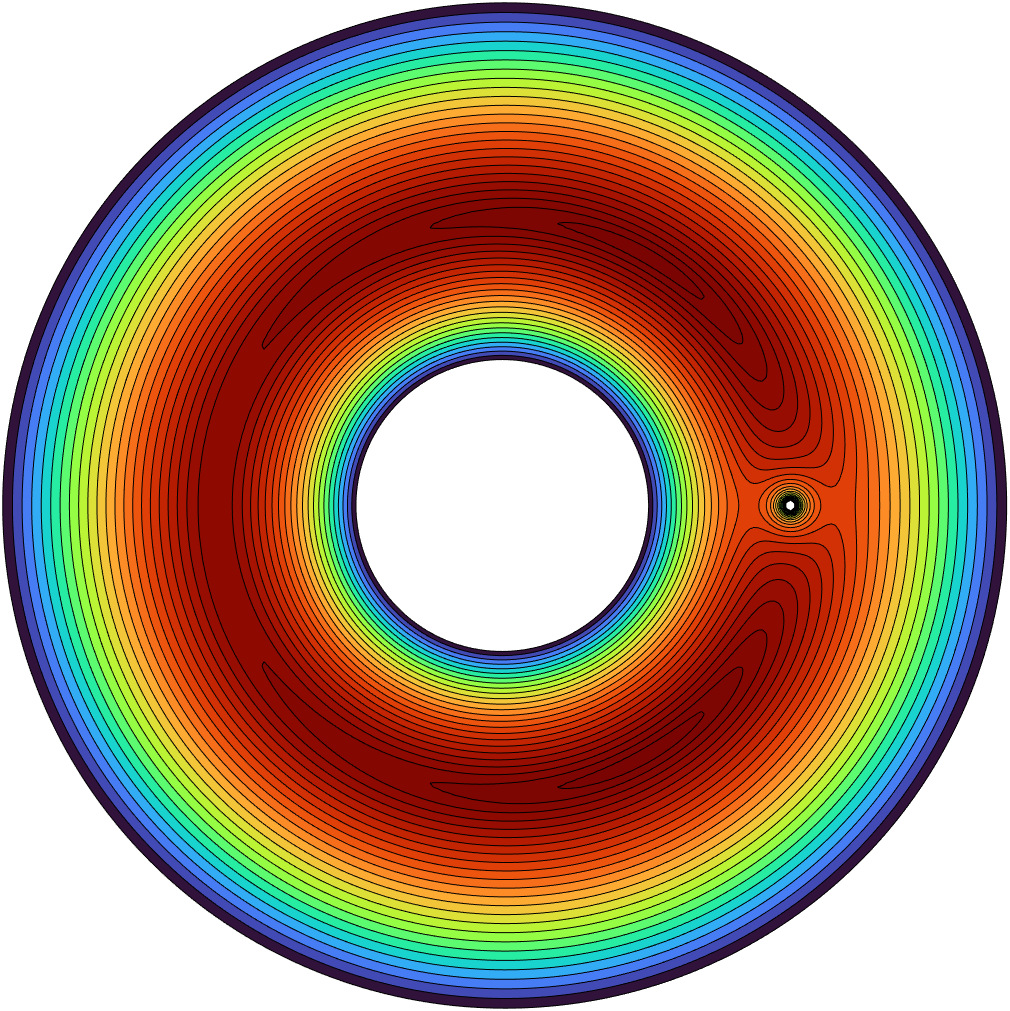
\includegraphics[width=0.4\textwidth]{level_curves/potential0.01.png}
\end{figure}
\begin{figure}[H]
    \caption{Level Curves of the pseudopotential for $\mu=0.1$}
    \centering
    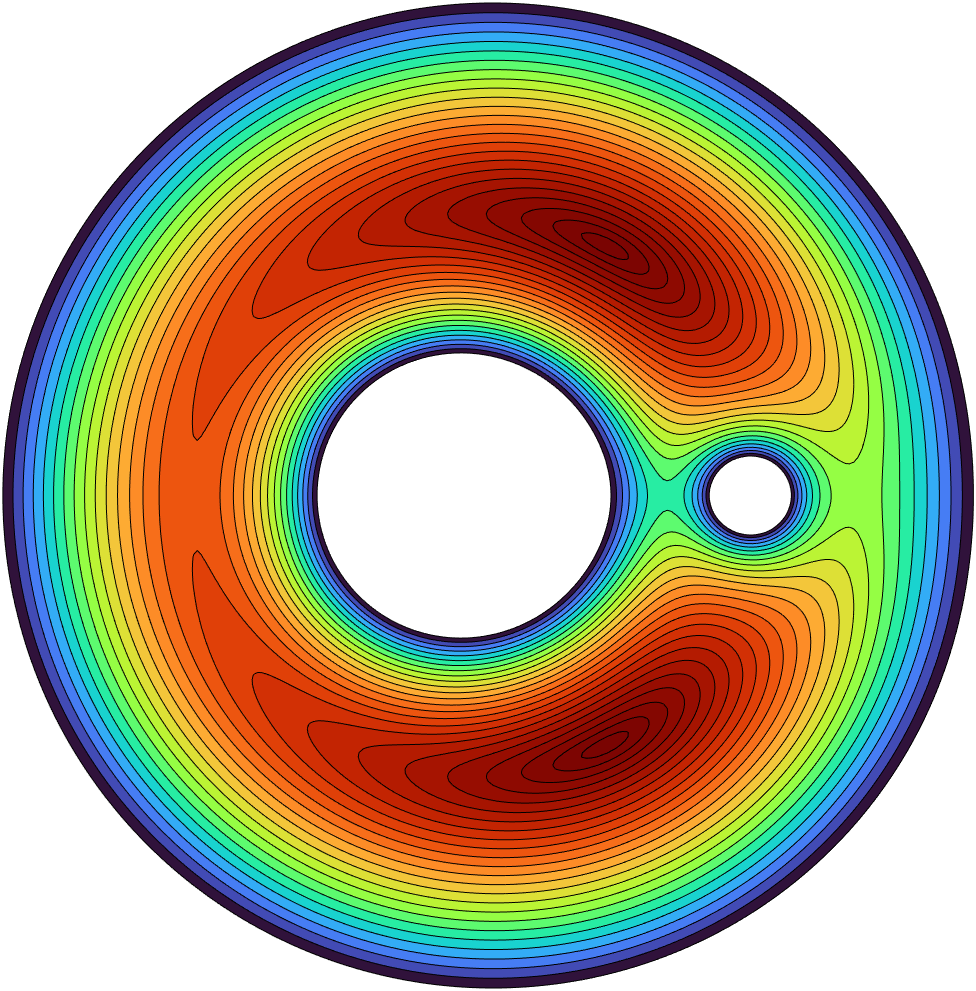
\includegraphics[width=0.4\textwidth]{level_curves/potential0.1.png}
\end{figure}
\begin{figure}[H]
    \caption{Level Curves of the pseudopotential for $\mu=0.25$}
    \centering
    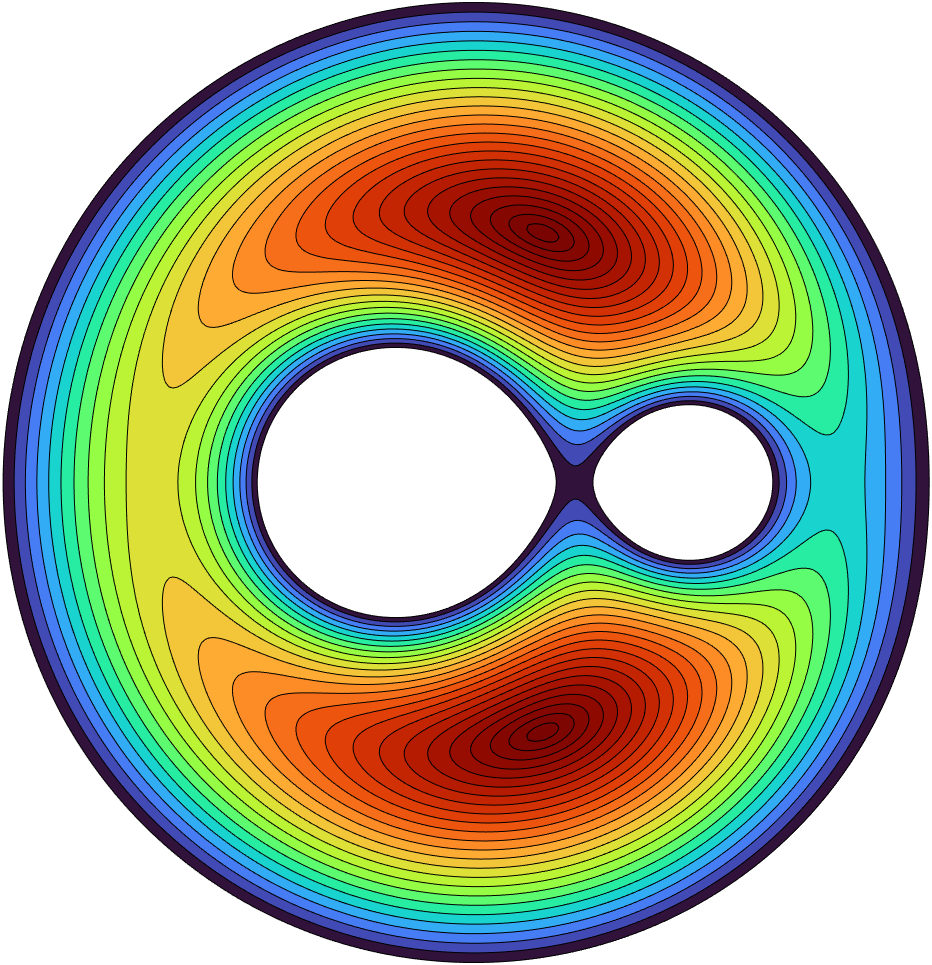
\includegraphics[width=0.4\textwidth]{level_curves/potential0.25.png}
\end{figure}
\begin{figure}[H]
    \caption{Level Curves of the pseudopotential for $\mu=0.5$}
    \centering
    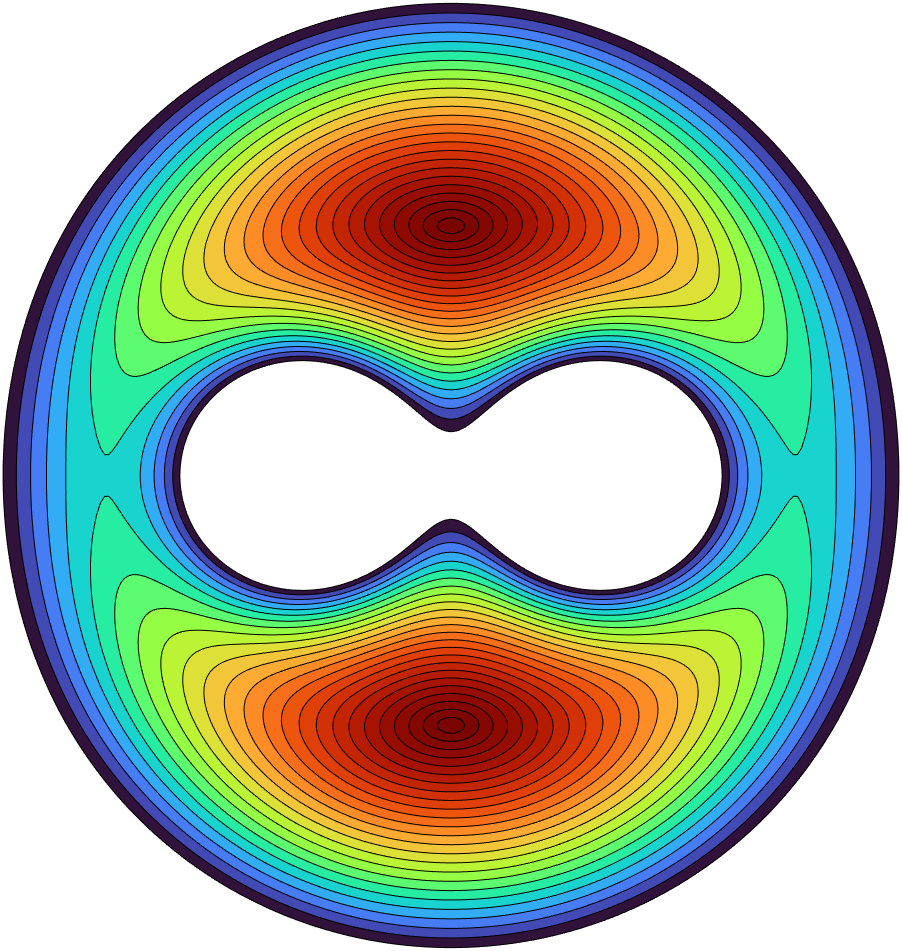
\includegraphics[width=0.4\textwidth]{level_curves/potential0.5.png}
\end{figure}

For reference, the mass ratio value $\mu$ for the Earth-Moon system is $\mu\approx0.012$, which is roughly that of the first diagram. Clearly, entering regions near the orbit of the second body is challenging, but exceeding those regions is quite feasible if done in the proximity of the secondary body.

\section*{Zero-Velocity Solutions - Lagrange Points}

There are some solutions for which the velocity is zero for all times, called Lagrange Points or libration points. To find these, we simply set the derivatives in the EOMs equal to zero.

\[\begin{aligned}
    \cancel{\ddot{x}}&=-\frac{1-\mu}{r_1^3}(x+\mu)-\frac{\mu}{r_2^3}(x-1+\mu)+\cancel{2\dot{y}}+x\\
    \cancel{\ddot{y}}&=-\frac{1-\mu}{r_1^3}y-\frac{\mu}{r_2^3}y-\cancel{2\dot{x}}+y\\
    \cancel{\ddot{z}}&=-\frac{1-\mu}{r_1^3}z-\frac{\mu}{r_2^3}z
\end{aligned}\]

Looking at the $z$ EOM, the right-hand-side must have the opposite sign to $z$. Therefore, for the velocity to remain zero, $z=0\forall t$. We will examine the case of $y=0$ and $y\ne0$ separately.

First, we look at $y=0$, which eliminates the second equality above.

\[\begin{aligned}
    \cancel{\ddot{x}}&=-\frac{1-\mu}{r_1^3}(x+\mu)-\frac{\mu}{r_2^3}(x-1+\mu)+\cancel{2\dot{y}}+x\\
    0&=-\frac{1-\mu}{\sqrt{(x+\mu)^2}^3}(x+\mu)-\frac{\mu}{\sqrt{(x-1+\mu)^2}^3}(x-1+\mu)+x\\
    0&=-\frac{1-\mu}{|x+\mu|^3}(x+\mu)-\frac{\mu}{|x-1+\mu|^3}(x-1+\mu)+x
\end{aligned}\]

This has three solutions, typically called $L_1$ (the solution between the two bodies), $L_2$ (the solution on the far side of the smaller body), and $L_3$ (the solution on the far side of the larger body).

Now, we examine $y\ne0$

\[\begin{aligned}
    \cancel{\ddot{y}}&=-\frac{1-\mu}{r_1^3}y-\frac{\mu}{r_2^3}y-\cancel{2\dot{x}}+y\\
    0&=-\frac{1-\mu}{r_1^3}y-\frac{\mu}{r_2^3}y+y\\
    0&=-\frac{1-\mu}{r_1^3}-\frac{\mu}{r_2^3}+1\\
    1&=\frac{1-\mu}{r_1^3}+\frac{\mu}{r_2^3}\\
    \frac{1-\mu}{r_1^3}&=1-\frac{\mu}{r_2^3}\\
\end{aligned}\]
Bringing in the equation for $x$,
\[\begin{aligned}
    0&=-\frac{1-\mu}{r_1^3}(x+\mu)-\frac{\mu}{r_2^3}(x-1+\mu)+x\\
    0&=-\left(1-\frac{\mu}{r_2^3}\right)(x+\mu)-\frac{\mu}{r_2^3}(x-1+\mu)+x\\
    0&=-(x+\mu)+\frac{\mu}{r_2^3}(x+\mu)-\frac{\mu}{r_2^3}(x+\mu)+\frac{\mu}{r_2^3}+x\\
    0&=-x-\mu+\frac{\mu}{r_2^3}+x\\
    0&=-\mu+\frac{\mu}{r_2^3}\\
    \frac{1}{r_2^3}&=1\\
    r_2&=1
\end{aligned}\]
Plugging this back into $\frac{1-\mu}{r_1^3}=1-\frac{\mu}{r_2^3}$,
\[\begin{aligned}
    \frac{1-\mu}{r_1^3}&=1-\frac{\mu}{r_2^3}\\
    \frac{1-\mu}{r_1^3}&=1-\mu\\
    \frac{1}{r_1^3}&=1\\
    r_1&=1\\
\end{aligned}\]

The conditions $r_1=r_2=1$ locate the final two Lagrange points, forming equilateral triangles with the line connecting the two bodies.
\[\begin{aligned}
    r_1&=r_2\\
    \sqrt{(x+\mu)^2+y^2}&=\sqrt{(x-1+\mu)^2+y^2}\\
    (x+\mu)^2+y^2&=(x-1+\mu)^2+y^2\\
    (x+\mu)^2&=(x-1+\mu)^2\\
    x^2+\mu^2+2x\mu&=x^2-2x+2x\mu+1-2\mu+\mu^2\\
    0&=-2x+1-2\mu\\
    2x&=1-2\mu\\
    x&=\frac{1}{2}-\mu\\
\end{aligned}\]
Plugging this once again into $r_1=\sqrt{(x+\mu)^2+y^2}=1$,
\[\begin{aligned}
    \sqrt{(x+\mu)^2+y^2}&=1\\
    \left(\frac{1}{2}-\mu+\mu\right)^2+y^2&=1\\
    \frac{1}{4}+y^2&=1\\
    y^2&=\frac{3}{4}\\
    y=\pm\frac{\sqrt{3}}{2}
\end{aligned}\]

The points $y=\pm\sqrt{3}/2$, $x=\frac{1}{2}-\mu$ locate $L_4$ and $L_5$.

The Lagrange points are therefore

\begin{framed}
\begin{center}
\begin{tabular}{ c c c }
     Point & $x$ & $y$ \\
     $L_1$ & Numeric Solution (see below) & 0\\
     $L_2$ & Numeric Solution (see below) & 0\\
     $L_3$ & Numeric Solution (see below) & 0\\
     $L_4$ & $\frac{1}{2}-\mu$ & $\frac{\sqrt{3}}{2}$ \\
     $L_5$ & $\frac{1}{2}-\mu$ & $\frac{\sqrt{3}}{2}$
\end{tabular}
\end{center}
\[L_{1,2,3}:\qquad-\frac{1-\mu}{|x_{L1,2,3}+\mu|^3}(x+\mu)-\frac{\mu}{|x-1+\mu|^3}(x-1+\mu)+x=0\]
\end{framed}

The Lagrange points are shown below for the Earth-Moon system ($\mu=0.01215$) as well as for the Pluto-Charon system ($\mu=0.10828$)0829

\begin{figure}[H]
    \def\muEM{0.01215058560962404}
    \centering
    \begin{tikzpicture}[
        planet/.style = {circle, draw=black, ball color=#1, node contents={}, inner sep = 0.1cm}, 
        point/.style = {circle, draw=#1, fill=#1, node contents={}, inner sep=0.05cm},
        >=latex
        ]

        \node (B1) at (-3*\muEM,0)     [planet=blue, label=below:Earth];
        \node (B2) at (3-3*\muEM,0)      [planet=gray, label=below:Moon];
        
        \draw[dash dot, fill=none, blue](0,0) circle (3*\muEM);
        \draw[dash dot, fill=none, gray](0,0) circle (3-3*\muEM);
        
        \node (L4) at (1.5-3*\muEM,{3*sqrt(3)/2}) [point=black, label=right:$L_4$];
        \node (L5) at (1.5-3*\muEM,{-3*sqrt(3)/2}) [point=black, label=right:$L_5$];
        \node (L1) at (3*0.8369151,0) [point=black, label=left:$L_1$];
        \node (L2) at (3*1.1556822,0) [point=black, label=right:$L_1$];
        \node (L3) at (3*-1.0050626,0) [point=black, label=left:$L_1$];

    \end{tikzpicture}

    \caption{Earth-Moon Lagrange Points. Earth-Moon barycenter is within Earth}
\end{figure}

\begin{figure}[H]
    \def\muEM{0.10829}
    \centering
    \begin{tikzpicture}[
        planet/.style = {circle, draw=black, ball color=#1, node contents={}, inner sep = 0.1cm}, 
        point/.style = {circle, draw=#1, fill=#1, node contents={}, inner sep=0.05cm},
        >=latex
        ]

        \node (B1) at (-3*\muEM,0)     [planet=orange, label=below:Pluto];
        \node (B2) at (3-3*\muEM,0)      [planet=brown, label=below:Charon];
        
        \draw[dash dot, fill=none, orange](0,0) circle (3*\muEM);
        \draw[dash dot, fill=none, brown](0,0) circle (3-3*\muEM);
        
        \node (L4) at (1.5-3*\muEM,{3*sqrt(3)/2}) [point=black, label=right:$L_4$];
        \node (L5) at (1.5-3*\muEM,{-3*sqrt(3)/2}) [point=black, label=right:$L_5$];
        \node (L1) at (3*0.59345355,0) [point=black, label=left:$L_1$];
        \node (L2) at (3*1.26244918,0) [point=black, label=right:$L_1$];
        \node (L3) at (3*-1.0450471,0) [point=black, label=left:$L_1$];

    \end{tikzpicture}

    \caption{Pluto-Charon Lagrange Points}
\end{figure}

\section*{CR3BP Canonical Dynamics}

Now that you are familiar with the governing equations of CR3BP dynamics, canonical behavior can be explored. First, a qualitative note:

\begin{framed}
Motion in the rotating frame acts as "feels" natural under gravitational influence, except for two effects.
\begin{enumerate}
    \item Centripedal acceleration causes objects to accelerate outward proportionally to their distance from the barycenter.
    \item The Coriolis acceleration causes objects to curve counterclockwise (when viewed from above) proportionally to their velocity.
\end{enumerate}
\end{framed}

With what little intuition that can be established having been addressed, canonical families of orbits in the CR3BP can be examined.

In Keplerian mechanics, the space of all possible orbits is five-dimensional (uniquely determined by semimajor axis, inclination, eccentricity, right ascension of ascending node, and and argument of periapsis) with few degenerate cases (such as circular or equatorial orbits) that remove dimensions. Furthermore, all initical conditions in Keplerian dynamics lead to periodic solutions. These are  not the case of CR3BP dynamics. The constraint of periodicity enforces many requirements on initial conditions, leading to a single-dimensional continuum of periodic orbits where any exist at all. Conventionally, these orbits are broken into a few different "families".

\newpage
Note that I consulted many references during the making of this. Where applicable, specific references are cited.
\nocite{*}
\bibliographystyle{IEEEtran} % We choose the "plain" reference style
\bibliography{refs} % Entries are in the refs.bib file

\end{document}